\documentclass[8pt]{amsart}
\usepackage{amsmath, amssymb}
\usepackage{amsfonts}
\usepackage{mathrsfs}
\usepackage[arrow,matrix,curve,cmtip,ps]{xy}
\usepackage{paralist}
\usepackage[left=1in,top=1in,right=1in,bottom=1in]{geometry}
\usepackage{amsthm}
\usepackage{tikz}
\usetikzlibrary{arrows,chains,matrix,positioning,scopes}

\allowdisplaybreaks

\theoremstyle{plain}% default

\theoremstyle{definition}
\newtheorem{theorem}{Theorem}[section]
\newtheorem{lemma}{Lemma}[section]
\newtheorem*{proposition}{Proposition}
\newtheorem*{corollary}{Corollary}
\newtheorem*{KL}{Klein’s Lemma}

\newtheorem*{definition}{Definition}
\newtheorem{conjecture}{Conjecture}[section]
\newtheorem{example}{Example}[section]
\newtheorem*{exercise}{Exercise}%[section]
\newtheorem*{notation}{Notation}
\newtheorem*{remark}{Remark}

\theoremstyle{remark}
\newtheorem*{note}{Note}
\newtheorem{case}{Case}

%this has equations numbered within sections 1.1,1.2, ... 2.1,...
\numberwithin{equation}{section}

\makeatletter
\newenvironment{solution}
               {\let\oldqedsymbol=\qedsymbol%
                \def\@addpunct##1{}%
                \renewcommand{\qedsymbol}{$\blacktriangleleft$}%
                \begin{proof}[\itshape Solution.]}%
               {\end{proof}%
                \renewcommand{\qedsymbol}{\oldqedsymbol}}
\makeatother

\makeatletter
\tikzset{join/.code=\tikzset{after node path={%
\ifx\tikzchainprevious\pgfutil@empty\else(\tikzchainprevious)%
edge[every join]#1(\tikzchaincurrent)\fi}}}
\makeatother

\tikzset{>=stealth',every on chain/.append style={join},
         every join/.style={->}}




\def\upint{\mathchoice%
    {\mkern13mu\overline{\vphantom{\intop}\mkern7mu}\mkern-20mu}%
    {\mkern7mu\overline{\vphantom{\intop}\mkern7mu}\mkern-14mu}%
    {\mkern7mu\overline{\vphantom{\intop}\mkern7mu}\mkern-14mu}%
    {\mkern7mu\overline{\vphantom{\intop}\mkern7mu}\mkern-14mu}%
  \int}
\def\lowint{\mkern3mu\underline{\vphantom{\intop}\mkern7mu}\mkern-10mu\int}


%-------------------------------------------
%       Begin Local Macros
%-------------------------------------------

\newcommand{\Z}{\mathbb{Z}}
\newcommand{\N}{\mathbb{N}}
\newcommand{\Q}{\mathbb{Q}}
\newcommand{\R}{\mathbb{R}}
\newcommand{\C}{\mathbb{C}}
\newcommand{\T}{\mathbb{T}}
\newcommand{\D}{\displaystyle}
\newcommand{\im}{\operatorname{im}}
\newcommand{\coker}{\operatorname{coker}}
\newcommand{\obj}{\operatorname{obj}}
\newcommand{\Hom}{\operatorname{Hom}}
\newcommand{\Mod}{\operatorname{\textbf{Mod}}}
\newcommand{\ind}{\operatorname{ind}}
\newcommand{\rank}{\operatorname{rank}}
\newcommand\mc[1]{\marginpar{\sloppy\protect\footnotesize #1}}

%-------------------------------------------
%       End Local Macros
%-------------------------------------------
\begin{document}
\title[MATH 697]{Introduction to Homological Algebra}

% \author{Robert Cardona}

\author{
	Robert Cardona %\textit{mrrobertcardona@gmail.com}
	\and
	Massy Khoshbin %\textit{massy255@gmail.com}
	\and
	Siavash Mortezavi %\textit{siavash.mortezavi@gmail.com}
}


\address{Department of Mathematics \\ California State University Long Beach}
\email{mrrobertcardona@gmail.com \and massy255@gmail.com \and siavash.mortezavi@gmail.com}

\date{\today}


\maketitle

%%%%%%%%%%%%%%%%%%%%%%%%%%%%%%%%%%%%%%%%%%%%%%%%
\setcounter{section}{0}
\section{MATH 697 Notes}
%%%%%%%%%%%%%%%%%%%%%%%%%%%%%%%%%%%%%%%%%%%%%%%%

\textbf{AM Proposition 1.1}: There is a one-to-one order-preserving correspondence between the ideals $I$ of $R$ which contain $(r)$ and the ideals $\overline I$ of $R/(r)$.
	\begin{proof}
		Define $\varphi : \{ I$ ideal of $R : (r) \subseteq I\} \to \{\overline I : \overline I$ is an ideal of $R/(r)\}$ by $\varphi(I) = I + (r)$. We must first show that this mapping is well defined, i.e., does $\varphi$ in fact map into an ideal of $R/(r)$? Say $I$ is an ideal of $R$ with $(r) \subseteq I$. Consider $\varphi(I) = I + (r)$. Choose $t \in R$ arbitrary and conclude that $[s + (r)][I + (r)] = sI + (r)$ but since $I$ is an ideal of $R$, $sI = I$ so $[s + (r)][I + (r)] = sI + (r) = [s + (r)] \overline I \subseteq \overline I$. Hence $\varphi$ is in fact well-defined.\\

		Now we want to show that $\varphi$ is surjective. Choose $\overline I$ an ideal of $R/(r)$. Does there exist an ideal $I$ of $R$ containing $(r)$ such that $\varphi(I) = \overline I$? Since $\overline I$ is an ideal of $R/(r)$, it follows that $\overline I = \{s + (r) : $ for some $s \in R\}$. Define $I = \{s\}$ where $s$ comes from previous definition. Is this in fact an ideal of $R$? Well we need to first show that it is an additive subgroup:
		\begin{enumerate}
			\item Observe that $0 \in \overline I$ since $(r) \in \overline I$. so $0 \in I$ so $I \neq \emptyset$.
			\item Let $s, t \in I$, Then $s + t + (r) = [s + (r)] + (t + (r)] \in \overline I$ since $\overline I$ is closed under addition. So $s + t \in I$.
			\item Let $s \in I$, then $s + (r) \in \overline I$ and since $\overline I$ is an additive subgroup it follows that $-s + (r) \in \overline I$ so $-s \in I$.
		\end{enumerate}
		Conclude by definition of subgroup that $I$ is in fact an additive subgroup. Now we must show that $I$ is closed under multiplication. Say $t \in R$, is $ts \in I$? well observe that since $s + (r) \in \overline I$ and $\overline I$ is an ideal, it follows that $t[s+ (r)] = ts + t(r) = ts + (r) \in \overline I$ so it follows that $ts \in I$. Conclude that $I$ is in fact an ideal. Now we must ask, is $(r) \subseteq I$? Let $x \in (r)$ then $x = rt$ for some $t \in R$. So $rs + (r) = 0 + (r) \in \overline I$. So it follows that $(r) \subseteq I$. Now $\varphi(I) = I + (r) = \overline I$ so $\varphi$ is in fact surjective.\\

		Now we must show that $\varphi$ is injective. Suppose that $\varphi(I) = \overline 0 = 0 + (r) = (r)$. Then since $\varphi(I) = I + (r) = 0 + (r)$ it follows that $I \subseteq (r)$. But since we know $(r) \subseteq I$ it follows that $I + (r)$ which is our \textit{zero} in this case. Conclude that $\varphi$ is in fact injective.\\

		\textit{Alternate Injective Proof}: Suppose that $\varphi(I_1) = \varphi(I_2)$ then we have $I_1 + (r) = I_2 + (r)$ but by property of cosets we have $I_1 - I_2 = (r)$ but this is the same as $I_1 + I_2 = (r)$ by way of just absorbing the negative sign (being an ideal). But since $(r) \subseteq I_1$ and $(r) \subseteq I_2$ it follows that $I_1 = I_2$. Conclude that $\varphi$ is injective.\\

		Now we must show that order is preserved. Suppose $I_1 \subseteq I_2$. We want to show that $\varphi(I_1) \subseteq \varphi(I_2)$. Say $x + (r) \in \varphi(I_1)$ then it follows that $x \in I_1 = I_2$ so immediately $x + (r) \in I_2 + (r) = \varphi(I_2)$. Conclude result.

	\end{proof}

\textbf{R Proposition 2.18}:
	\begin{enumerate}
		\item A sequence $0 \rightarrow A \xrightarrow{f} B$ is exact if and only if $f$ is injective.
		\item A sequence $B \xrightarrow g C \rightarrow 0$ is exact if and only if $g$ is surjective.
		\item A sequence $0 \rightarrow A \xrightarrow{h} B \rightarrow 0$ is exact if and only if $h$ is an isomorphism.
	\end{enumerate}

\textbf{DF \S10.5 Proposition 24}: (\textit{The Short Five Lemma}) Let $\alpha, \beta, \gamma$ be homomorphisms of short exact sequences:\\

	\begin{center}
	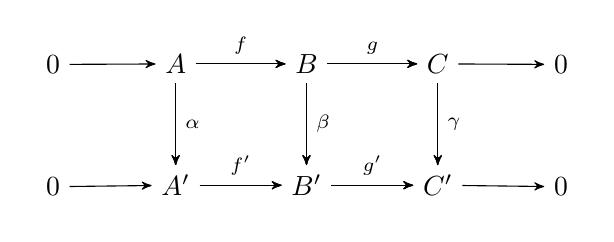
\begin{tikzpicture}
	  \matrix (m) [matrix of math nodes, row sep=3em, column sep=3em]
	    { 0 & A  & B  & C  & 0 \\
	      0 & A' & B' & C' & 0 \\ };
	  { [start chain] \chainin (m-1-1);
	    \chainin (m-1-2);
	    { [start branch=A] \chainin (m-2-2)
	        [join={node[right] {$\scriptstyle\alpha$}}];}
	    \chainin (m-1-3) [join={node[above] {$\scriptstyle f$}}];
	    { [start branch=B] \chainin (m-2-3)
	        [join={node[right] {$\scriptstyle\beta$}}];}
	    \chainin (m-1-4) [join={node[above] {$\scriptstyle g$}}];
	    { [start branch=C] \chainin (m-2-4)
	        [join={node[right] {$\scriptstyle\gamma$}}];}
	    \chainin (m-1-5); }
	  { [start chain] \chainin (m-2-1);
	    \chainin (m-2-2);
	    \chainin (m-2-3) [join={node[above] {$\scriptstyle f'$}}];
	    \chainin (m-2-4) [join={node[above] {$\scriptstyle g'$}}];
	    \chainin (m-2-5); }
	\end{tikzpicture}
	\end{center}

	\begin{enumerate}
		\item If $\alpha$ and $\gamma$ are injective then so is $\beta$.
			\begin{proof}
				Let $b \in B$ such that $\beta(b) = 0$. We want to show that $b = 0$. Observe that $g'(\beta(b)) = g'(0) = 0$. By commutativity we have $\gamma(g(b)) = g'(\beta(b)) = g'(0) = 0$. Since $\gamma$ is injective we know $g(b) = 0$ so $b \in \ker g$ but since we are in an exact sequence we have $\im f = \ker g$ and hence $b \in \im f$. By definition there exists $a \in A$ with $f(a) = b$. Now $f'(\alpha(a)) = \beta(f(a)) = \beta(b) = 0$. Since $f'$ is injective, it follows that $\alpha(a) = (f')^{-1}(0) = 0$. Now we have $a = \alpha^{-1}(0)$ and so $a = 0$. So $0 = f(a) = b$.
			\end{proof}
		\item If $\alpha$ and $\gamma$ are surjective then so is $\beta$.
			\begin{proof}
				Let $b' \in B'$ then $g'(b') \in C'$. Since $\gamma$ is surjective there excists $c \in C$ such that $\gamma(c) = g'(b')$. Since this is an exact sequence, $g$ is surjective so there exists $b \in B$ such that $g(b) = c$. By equality we have $\gamma(c) = \gamma(g(b)) = g'(b')$. Now observe that $$g'(b' - \beta(b)) = g'(b') - g'(\beta(b)) = g'(b') - \gamma(g(b)) = g'(b') - g'(b') = 0$$ So in particular $b' - \beta(b) \in \ker g'$ but by exactness $\im f' = \ker g'$ so there exists $a' \in A'$ such that $f'(a') = b' - \beta(b)$. But since $\alpha$ is surjective, there exists $a \in A$ such that $\alpha(a) = a'$. Now $f'(a') = f'(\alpha(a)) = b' - \beta(b)$. By commutativity $f'(\alpha(a)) = \beta(f(a)) = b' - \beta(b)$ so $\beta(f(a)) + \beta(b) = b'$ and we have $\beta(f(a) + b) = b'$.
			\end{proof}
		\item If $\alpha$ and $\gamma$ are isomorphisms then so is $\beta$ (and then the two sequences are isomorphism).
			\begin{proof}
				Follows from $(1)$ and $(2)$.\\
			\end{proof}
	\end{enumerate}

\textbf{R Proposition 2.72}: (\textit{Five Lemma}) Consider the commutative diagram with exact rows.
	\begin{center}
	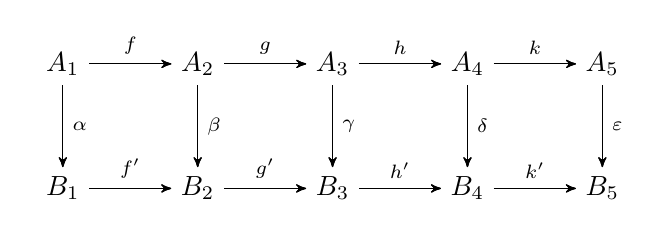
\begin{tikzpicture}
	  \matrix (m) [matrix of math nodes, row sep=3em, column sep=3em]
	    { A_1 & A_2  & A_3  & A_4  & A_5 \\
	      B_1 & B_2 & B_3 & B_4 & B_5 \\ };
	  { [start chain] 
	    \chainin (m-1-1);
	    { [start branch=A] \chainin (m-2-1)
	        [join={node[right] {$\scriptstyle\alpha$}}];}

	    \chainin (m-1-2)  [join={node[above] {$\scriptstyle f$}}];
	    { [start branch=B] \chainin (m-2-2)
	        [join={node[right] {$\scriptstyle\beta$}}];}

	    \chainin (m-1-3) [join={node[above] {$\scriptstyle g$}}];
	    { [start branch=C] \chainin (m-2-3)
	        [join={node[right] {$\scriptstyle\gamma$}}];}

	    \chainin (m-1-4) [join={node[above] {$\scriptstyle h$}}];
	    { [start branch=D] \chainin (m-2-4)
	        [join={node[right] {$\scriptstyle\delta$}}];}

	    \chainin (m-1-5)  [join={node[above] {$\scriptstyle k$}}];}
  	    { [start branch=E] \chainin (m-2-5)
	        [join={node[right] {$\scriptstyle\varepsilon$}}];}

	  { [start chain] \chainin (m-2-1);
	    \chainin (m-2-2) [join={node[above] {$\scriptstyle f'$}}];
	    \chainin (m-2-3) [join={node[above] {$\scriptstyle g'$}}];
	    \chainin (m-2-4) [join={node[above] {$\scriptstyle h'$}}];
	    \chainin (m-2-5) [join={node[above] {$\scriptstyle k'$}}]; }
	\end{tikzpicture}
	\end{center}

	\begin{enumerate}
		\item If $\beta$ and $\delta$ are surjective and $\varepsilon$ is injective, then $\gamma$ is surjective.
		\item If $\beta$ and $\delta$ are injective and $\alpha$ is surjective, then $\gamma$ is injective.
		\item If $\alpha, \beta, \delta$ and $\varepsilon$ are isomorphisms, then $\gamma$ is an isomorphism.
	\end{enumerate}

\textbf{R Exercise 2.14}: Let $A \xrightarrow f B \xrightarrow g C$ be a sequence of module maps. Prove that $gf = 0$ if and only if $\im f \subseteq \ker g$.  Give an example of such a sequence that is not exact.
	\begin{proof}
		Suppose $gf = 0$, that is, $f(g(a)) = 0$ for all $a \in A$. Let $b \in \im f$ then by definition there exists $a \in A$ such that $f(a) = b$. But we know by hypothesis that $0 = g(f(a)) = g(b)$ so $b \in \ker g$. Conclude that $\im f \subseteq \ker g$. Conversely, suppose that $\im f \subseteq \ker g$. Let $a \in A$ and observe that $f(a) \in \im f$. By hypothesis $f(a) \in \ker g$ so $g(f(a)) = 0$. Since $a$ was arbitrary conclude $gf = 0$.
	\end{proof}
	Consider the sequence of module maps $\Z/4\Z \xrightarrow f \Z/3\Z \xrightarrow g \Z/2\Z$ where $f(\overline x) = 2 \overline x$ and $g(\overline y) = \overline y$. Observe that $\im f = \Z/3\Z$  and $\ker g = \{0\}$. Since $\im f \neq \ker g$ it follows that this is \textbf{not} an exact sequence.\\

\textbf{R Exercise 2.15}:
	\begin{enumerate}
		\item Prove that $f : M \to N$ is surjective if and only if $\coker f = \{0\}$.
			\begin{proof}
				Suppose $f : M \to N$ is surjective then for $n \in N$, there exists $m \in M$ such that $f(m) = n$. By definition $\coker f = M/\im f = M/M = 0$. Conversely, suppose that $\coker f = 0$, i.e., $M/\im f = 0$ implying that if $m + \im f \in M/\im f$ then $m + \im f = 0$ or equivalently $m \in \im f$. Since $m$ is arbitrary, conclude $M = \im f$ and hence $f$ is surjective by definition.
			\end{proof}
		\item If $f : M \to N$ is a map, prove that there is an exact sequence $$ 0 \rightarrow \ker f \rightarrow M \xrightarrow f N \rightarrow \coker f \rightarrow 0.$$
			\begin{proof}
				Define $h : \ker f \to M$ by $h(m) = m$, that is, map each element to itself. It follows immediately that $\im h = \ker f$. Define $g : N \to \coker f = N/\im f$ by $g(n) = n + \im f$, that is, the canonical/projection mapping. Observe that $\ker g = \im f$. Conclude that the following sequence is in fact exact: $$0 \xrightarrow{\text{identity}} \ker f \xrightarrow h M \xrightarrow f N \xrightarrow g \coker f \xrightarrow{\text{zero}} 0. \qedhere$$
			\end{proof}
	\end{enumerate}

\textbf{R Exercise 2.16}:
	\begin{enumerate}
		\item If $0 \rightarrow M \rightarrow 0$ is an exact sequence, prove that $M = \{0\}$.
			\begin{proof}
				Consider $0 \xrightarrow f M \xrightarrow g 0$. Since $f$ is surjective then for $m \in M$ there exists $x \in 0$ such that $f(x) = m$ but $x$ must be $0$ so $m = 0$.
			\end{proof}
		\item If $A \xrightarrow f B \xrightarrow g C \xrightarrow h D$ is an exact sequence, prove that $f$ is surjective if and only if $h$ is injective.
			\begin{proof}
				Suppose $f$ is surjective. Then $\im f = B = \ker g$ but this immediately implies that $\im g = 0 = \ker h$ so $h$ is injective by definitoin. Conversely, suppose $h$ is injective. Then $\ker h = 0 = \im g$ which immediately implies $\ker g = B = \im f$. Conclude by definition $f$ is surjective.
			\end{proof}
		\item Let $A \xrightarrow \alpha B \xrightarrow \beta C \xrightarrow \gamma D \xrightarrow \delta E$ be exact. If $\alpha$ and $\delta$ are isomorphisms, prove that $C = \{0\}$.
			\begin{proof}
				Observe that, by previous exercise, $\beta$ is surjective and $\gamma$ is injective so we have $\im \beta = C$ and $\ker \gamma = 0$. Result follows by exactness: $C = \im \beta = \ker \gamma = 0$. Conclude $C = \{0\}$.
			\end{proof}
	\end{enumerate}




\textbf{R Exercise 2.17}: If $A \xrightarrow f B \xrightarrow g C \xrightarrow h D \xrightarrow k E$ is exact, prove that there is an exact sequence $0 \rightarrow \coker f \xrightarrow \alpha C \xrightarrow \beta \ker k \rightarrow 0$, where $\alpha : b + \im f \mapsto g(b)$ and $\beta : c \mapsto h(c)$.
	\begin{proof}
		Observe that $\ker \beta = \{c \in C : \beta(c) = h(c) = 0\} = \ker h = \im g$ by exactness and since $\alpha$ can run through any $b \in B$ conclude $\im \alpha = \im g = \ker \beta$
	\end{proof}



\textbf{R Exercise 2.32}: (\textit{$3 \times 3$ Lemma}) Consider the following commutative diagram in $_R\Mod$ having exact columns.
	\begin{center}
	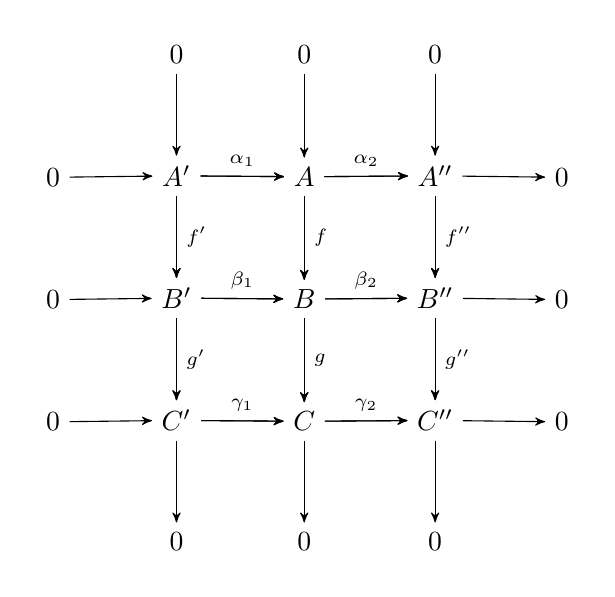
\begin{tikzpicture}

	\matrix (m) [matrix of math nodes, row sep=3em, column sep=3em]
	  {  & 0  & 0 & 0   & \\
	   0 & A' & A & A'' & 0\\
	   0 & B' & B & B'' & 0\\
	   0 & C' & C & C'' & 0\\
	     & 0  & 0 & 0   & \\};
	{ [start chain] \chainin (m-1-2); { [start branch = A] \chainin (m-2-2); } }
	{ [start chain] \chainin (m-1-3); { [start branch = B] \chainin (m-2-3); } }
	{ [start chain] \chainin (m-1-4); { [start branch = C] \chainin (m-2-4); } }
	{ [start chain] 
		\chainin (m-2-1);
		\chainin (m-2-2); 
			{ [start branch = D] \chainin (m-3-2) [join = {node[right] {$\scriptstyle f'$}}]; } 
		\chainin (m-2-3) [join = {node[above] {$\scriptstyle \alpha_1$}}];
			{ [start branch = E] \chainin (m-3-3) [join = {node[right] {$\scriptstyle f$}}]; }
		\chainin (m-2-4) [join = {node[above] {$\scriptstyle \alpha_2$}}];
			{ [start branch = F] \chainin (m-3-4) [join = {node[right] {$\scriptstyle f''$}}]; }
		\chainin (m-2-5);
	}
	{ [start chain] 
		\chainin (m-3-1);
		\chainin (m-3-2); 
			{ [start branch = G] \chainin (m-4-2) [join = {node[right] {$\scriptstyle g'$}}]; } 
		\chainin (m-3-3) [join = {node[above] {$\scriptstyle \beta_1$}}];
			{ [start branch = H] \chainin (m-4-3) [join = {node[right] {$\scriptstyle g$}}]; }
		\chainin (m-3-4) [join = {node[above] {$\scriptstyle \beta_2$}}];
			{ [start branch = I] \chainin (m-4-4) [join = {node[right] {$\scriptstyle g''$}}]; }
		\chainin (m-3-5);
	}
	{ [start chain] 
		\chainin (m-4-1);
		\chainin (m-4-2); 
			{ [start branch = J] \chainin (m-5-2); } 
		\chainin (m-4-3) [join = {node[above] {$\scriptstyle \gamma_1$}}];
			{ [start branch = K] \chainin (m-5-3); }
		\chainin (m-4-4) [join = {node[above] {$\scriptstyle \gamma_2$}}];
			{ [start branch = L] \chainin (m-5-4); }
		\chainin (m-4-5);
	}	
	\end{tikzpicture}
	\end{center}

	If the bottom two rows are exact, prove that the top row is exact; if the top two rows are exact, prove that the bottom row is exact.

	\begin{proof}
		Suppose that the bottom two rows are exact. We must show four things:
		\begin{enumerate}
			\item $\boxed{\alpha_1$ is injective$}$: Suppose $a' \in A'$ with $\alpha_1(a') = 0$. Observe that by commutativity $f(\alpha_1(a')) = \beta_1(f'(a')) = 0$ so since $\beta_1$ is injective, by exactness of the second row, $f'(a') = 0$. But since the first column is exact by hypothesis, we have $a' = 0$. Conclude that $\alpha_1$ is in fact injective.
			\item $\boxed{\im \alpha_1 \subseteq \ker \alpha_2}$: Choose $a \in \im \alpha_1$ then by definition there exists $a' \in A'$ such that $\alpha_1(a') = a$. Observe that $f(a) = f(\alpha_1(a')) = \beta_1(f'(a'))$ by commutativity. Moreover $\beta_2(f(a)) = f''(\alpha_2(a))$ again by commutativity. Hence we have $$\beta_2(f(a)) = \beta_2(\beta_1(f'(a'))) = 0 = f''(\alpha_2(a)).$$ Since $f''$ is injective by exactness of the third column, $\alpha_2(a) = 0$ and so $a \in \ker \alpha_2$. Conclude that $\im \alpha_2 \subseteq \ker \alpha_2$ as desired.
			\item $\boxed{\ker \alpha_2 \subseteq \im \alpha_1}$: Let $a \in \ker \alpha_2$ then by definition $\alpha_2(a) = 0$ and so $f''(\alpha(a)) = \beta_2(f(a)) = 0$. So $f(a) \in \ker \beta_2 = \im \beta_1$ by exactness of the second column, so there exists $b' \in B'$ such that $\beta_1(b') = f(a)$. Now $$\gamma_1(g'(b)) = g(\beta_1(b')) = g(f(a)) = 0$$ by commutativity and exactness so there exists $a' \in A'$ such that $f'(a') = b'$. Now by commutativity $$f(\alpha_1(a')) = \beta_1(f'(a')) = \beta_1(b') = f(a)$$ and so $f(a - \alpha_1(a')) = 0$ since $f$ is a homomorphism. $f$ is injective since the second column is exact so it follows that $\alpha_1(a') = a$ and so $a \in \im \alpha_1$. Conclude that $\ker \alpha_2 \subseteq \im \alpha_1$ is in fact true.
			\item $\boxed{\alpha_2$ is surjective$}$: Choose $a'' \in A''$. Consider $f''(a'') \in B''$. Since the second row is exact $\beta_2$ is surjective so there exists $b \in B$ such that $\beta_2(b) = f''(a'')$. By commutativity $g''(\beta_1(b)) = \gamma_2(g(b))$ but by exactness of the third column $g''(\beta_2(b)) = g''(f''(a'')) = 0$. So $\gamma_2(g(b)) = 0$ which implies that $g(b) \in \ker \gamma_2 = \im \gamma_1$ by exactness of the third row. So there exists $c' \in C'$ such that $\gamma_1(c') = g(b)$. Since the first column is exact $g'$ is surjective so there exists $b' \in B'$ such that $g'(b') = c'$. So $\gamma_1(c') = \gamma_1(g'(b')) = g(\beta_1(b'))$. Observe that $$g(b - \beta_1(b')) = g(b) - g(\beta_1(b')) = 0$$ since $g(b) = \gamma_1(c)$ and $g(\beta_1(b')) = \gamma_1(c)$ also. So $b - \beta_1(b') \in \ker g = \im f$ by exactness of the second column. So there exists $a \in A$ such that $f(a) = b - \beta_2(b')$. Now since $f''(\alpha(a)) = \beta_2(f(a)) = \beta_2(b - \beta_1(b'))$ we get $$f''(\alpha_2(a)) = \beta_2(b) - \beta_2(\beta_1(b')) = \beta_2(b) = f''(a'').$$ In particular we get $f''(\alpha_2(a) - a'') = 0$ but $f''$ is injective by exactness of the third column so $\alpha_2(a) = a''$. Conclude that $\alpha_2$ is in fact surjective.
		\end{enumerate}
		We have shown that if the bottom two rows are exact, then the top row is exact.\\

		Suppose that the top two rows are exact. We must show four things:
		\begin{enumerate}
			\item $\boxed{\gamma_1$ is injective$}$: Suppose $c' \in C'$  with $\gamma_1(c') = 0$. Since the first column is exact, $g'$ is surjective so there exists $b' \in B'$ such that $g'(b') = c'$. Now by commutativity $$0 = \gamma_1(c') = \gamma_1(g'(b')) = g(\beta_1(b')).$$ So $\beta_1(b') \in \ker g = \im f$ since the second row is exact. So there exists $a \in A$ such that $f(a) = \beta_1(b')$. But by commutativity $$f''(\alpha_2(a)) = \beta_2(f(a)) = \beta_2(\beta_1(b')) = 0$$ so $\alpha_2(a) = 0$. Since $f''$ is injective, because the third column is exact. Now $a \in \ker \alpha_2 = \im \alpha_1$ by exactness of the first row so there exists $a' \in A'$ such that $\alpha_2(a') = a$. Now $$f(a) = f(\alpha_1(a')) = \beta_1(f'(a')) = \beta_1(b')$$ So $\beta_1(f'(a') - b') = 0$. Since the second row is exact, $\beta_1$ is injective so $f'(a') - b = 0$. Hence $f'(a') = b'$. Taking $g'$ of both sides we get $$ 0 = g'(f'(a')) = g'(b') = c'.$$ Hence $\gamma_1$ is injective.
			\item $\boxed{\im \gamma_1 \subseteq \ker \gamma_2}$: Let $c \in \im \gamma_1$ then by definition there exists $c' \in C'$ such that $\gamma_1(c') = c$. Since the first column is exact $g'$ is surjective so there exists $b' \in B'$ such that $g'(b') = c'$. Observe that $$g(\beta_1(b')) = \gamma_1(g'(b')) = \gamma_1(c') = c$$ by commutativity. Again by commutativity we observe $$\gamma_2(c) = \gamma_1(g(\beta_1(b'))) = g''(\beta_1(\beta_1(b'))) = g''(0) = 0$$ and so $c \in \ker \gamma_2$. Conclude that $\im \gamma_1 \subseteq \ker \gamma_2$.
			\item $\boxed{\ker \gamma_2 \subseteq \im \gamma_1}$: Choose $c \in \ker \gamma_2$ then by definition $\gamma_2(c) = 0$. Since the second column is exact, $g$ is surjective. So there exists $b \in B$ such that $g(b) = c$. By commutativity $$g''(\beta_2(b)) = \gamma_2(g(b)) = \gamma_2(c) = 0.$$ So $\beta_2(b) \in \ker g'' = \im f''$ by exactness of the third column so there exists $a'' \in A''$ such that $f''(a'') = \beta_2(b)$. Since the first row is exact $\alpha_2$ is surjective so there exists $a \in A$ such that $\alpha_2(a) = a''$. Now $$\beta_2(f(a)) = f''(\alpha_2(a)) = f''(a'') = \beta_2(b)$$ so $\beta_2(f(a) - b) = 0$ which implies that $f(a) - b \in \ker \beta_2 = \im \beta_1$ by exactness of the second row. So there exists $b' \in B'$ such that $\beta_1(b') = f(a) - b'$. But now $$ \gamma_1(g'(b')) = g(\beta_1(b')) = g(f(a) - b) = g(f(a)) = g(b) = -c$$ yielding $\gamma_1(-g'(b')) = c$. So $c \in \im \gamma_1$ and we can conclude that $\ker \gamma_2 \subseteq \im \gamma_1$.
			\item $\boxed{\gamma_2$ is surjective$}$: Choose $c'' \in C''$. Since the third column is exact $g''$ is surjective so there exists $b'' \in B''$ such that $g''(b'') = c''$. But since the second row is exact $\beta_2$ is surjective so there exists $b \in B$ such that $\beta_2(b) = b''$. Now by commutativity $$c'' = g''(b'') = g''(\beta_2(b)) = \gamma_2(g(b)).$$ Conclude that $\gamma_2$ is in fact surjective.
		\end{enumerate}
		We have shown that if the top two rows are exact, then the bottom row is exact.
	\end{proof}






\textbf{AM Proposition 2.10}: (\textit{Snake Lemma}) Let

	\begin{center}
	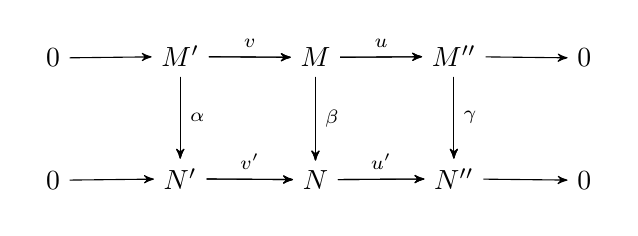
\begin{tikzpicture}
	  \matrix (m) [matrix of math nodes, row sep=3em, column sep=3em]
	    { 0 & M'  & M  & M''  & 0 \\
	      0 & N' & N & N'' & 0 \\ };
	  { [start chain] \chainin (m-1-1);
	    \chainin (m-1-2);
	    { [start branch=A] \chainin (m-2-2)
	        [join={node[right] {$\scriptstyle \alpha$}}];}
	    \chainin (m-1-3) [join={node[above] {$\scriptstyle v$}}];
	    { [start branch=B] \chainin (m-2-3)
	        [join={node[right] {$\scriptstyle \beta$}}];}
	    \chainin (m-1-4) [join={node[above] {$\scriptstyle u$}}];
	    { [start branch=C] \chainin (m-2-4)
	        [join={node[right] {$\scriptstyle \gamma$}}];}
	    \chainin (m-1-5); }
	  { [start chain] \chainin (m-2-1);
	    \chainin (m-2-2);
	    \chainin (m-2-3) [join={node[above] {$\scriptstyle v'$}}];
	    \chainin (m-2-4) [join={node[above] {$\scriptstyle u'$}}];
	    \chainin (m-2-5); }
	\end{tikzpicture}
	\end{center}

be a commutative diagram of $R$-modules and homomorphisms, with the rows exact. Then there exists a sequence $$0 \rightarrow \ker(\alpha) \xrightarrow{\overline v} \ker(\beta) \xrightarrow{\overline u} \ker (\gamma) \xrightarrow d \coker(\alpha) \xrightarrow {\overline v'} \coker (\beta) \xrightarrow{\overline u'} \coker(\gamma) \rightarrow 0$$ in which $\overline u$, $\overline v$ are restrictions of $u, v$, and $\overline u', \overline v'$ are induced by $u', v'$.\\

	\begin{proof}
	We consider: 	
	\begin{center}
	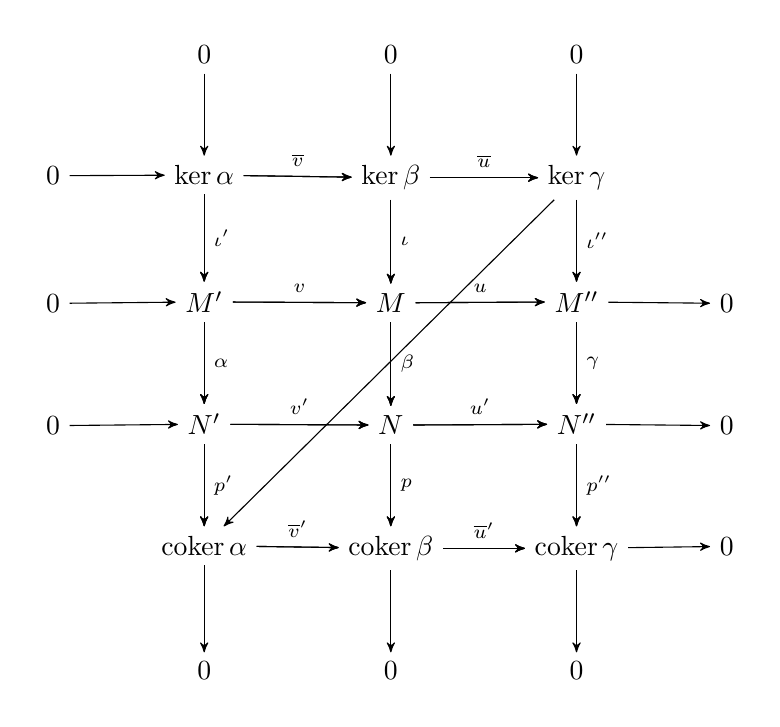
\begin{tikzpicture}

	\matrix (m) [matrix of math nodes, row sep=3em, column sep=3em]
	  {  & 0  & 0 & 0   & \\
	   0 & \ker \alpha & \ker \beta & \ker \gamma & \\
	   0 & M' & M & M'' & 0\\
	   0 & N' & N & N'' & 0\\
	   & \coker \alpha & \coker \beta & \coker \gamma & 0\\
	     & 0  & 0 & 0   & \\};
	{ [start chain] \chainin (m-1-2); { [start branch = A] \chainin (m-2-2); } }
	{ [start chain] \chainin (m-1-3); { [start branch = B] \chainin (m-2-3); } }
	{ [start chain] \chainin (m-1-4); { [start branch = C] \chainin (m-2-4); } }
	{ [start chain] 
		\chainin (m-2-1);
		\chainin (m-2-2); 
			{ [start branch = D] \chainin (m-3-2) [join = {node[right] {$\scriptstyle \iota'$}}]; } 
		\chainin (m-2-3) [join = {node[above] {$\scriptstyle \overline v$}}];
			{ [start branch = E] \chainin (m-3-3) [join = {node[right] {$\scriptstyle \iota$}}]; }
		\chainin (m-2-4) [join = {node[above] {$\scriptstyle \overline u$}}];
			{ [start branch = F] \chainin (m-3-4) [join = {node[right] {$\scriptstyle \iota''$}}]; }
		\chainin (m-5-2);
	}
	{ [start chain] 
		\chainin (m-3-1);
		\chainin (m-3-2); 
			{ [start branch = G] \chainin (m-4-2) [join = {node[right] {$\scriptstyle \alpha$}}]; } 
		\chainin (m-3-3) [join = {node[above] {$\scriptstyle v$}}];
			{ [start branch = H] \chainin (m-4-3) [join = {node[right] {$\scriptstyle \beta$}}]; }
		\chainin (m-3-4) [join = {node[above] {$\scriptstyle u$}}];
			{ [start branch = I] \chainin (m-4-4) [join = {node[right] {$\scriptstyle \gamma$}}]; }
		\chainin (m-3-5);
	}
	{ [start chain] 
		\chainin (m-4-1);
		\chainin (m-4-2); 
			{ [start branch = J] \chainin (m-5-2) [join = {node[right] {$\scriptstyle p'$}}]; } 
		\chainin (m-4-3) [join = {node[above] {$\scriptstyle v'$}}];
			{ [start branch = K] \chainin (m-5-3) [join = {node[right] {$\scriptstyle p$}}]; }
		\chainin (m-4-4) [join = {node[above] {$\scriptstyle u'$}}];
			{ [start branch = L] \chainin (m-5-4) [join = {node[right] {$\scriptstyle p''$}}]; }
		\chainin (m-4-5);
	}	
	{ [start chain] 
		\chainin (m-5-2); 
			{ [start branch = M] \chainin (m-6-2); } 
		\chainin (m-5-3) [join = {node[above] {$\scriptstyle \overline v'$}}];
			{ [start branch = N] \chainin (m-6-3); }
		\chainin (m-5-4) [join = {node[above] {$\scriptstyle \overline u'$}}];
			{ [start branch = O] \chainin (m-6-4); }
		\chainin (m-5-5);
	}	
	\end{tikzpicture}
	\end{center}

	Define $\overline v(x') = v(x')$, $\overline u(x) = u(x)$, $\overline v'(y' + \im \alpha) = v'(y') + \im \beta$, and $\overline u'(y + \im \beta) = u'(y) + \im \gamma$.\\

	For our definitions of $\overline v'$ and $\overline u'$ we must show that they are well defined. Consider $\overline v'$. Choose $\overline y' \in \coker \beta$ with $\overline y' = y' + \im \alpha$. Suppose $\overline y' = \overline z'$, then by property of cosets we have $y' - z' \in \im \alpha = \ker p'$ by exactness of first column. So $p'(y' - z') = 0$. Observe that $p(v'(y' - z')) = \overline v'(p'(y' - z')) = v'(0) = 0$ so $v(y' - z') \in \ker p= \im \beta$ by exactness of second column. In particular we have $v'(y') -v'(z') \in \im \beta$ and hence by property of cosets $$\overline v'(\overline y') = v'(y') + \im \beta = v'(z') + \im \beta = \overline v'(\overline z').$$ Conclude that the mapping is well defined. By similar reasoning we can show $\overline u'$ is well defined.\\

	Let $x'' \in \ker \gamma$ and consider $\iota''(x'') \in M''$. Since the second row is exact it follows that $u$ is surjective so there exists $m \in M$ such that $\boxed{u(m) = \iota''(m'')}$.By commutativity we get $$u'(\beta(m)) = \gamma(u(m)) = \gamma(\iota''(m'')) = \gamma(0) = 0.$$ So $\beta(m) \in \ker u' = \im v'$ by exactness of the third row. So there exists {\color{red} a unique?} $n' \in N'$ such that $\boxed{v'(n') = \beta(m)}$. Define $\boxed{d(x) = p'(n')}$. \\

We want to show that this mapping is well-defined, that is, we still get to the same place regardless of how we choose $m$ such that $u(m) = \iota''(m'')$. Suppose $u (\overline m) = u(m) = \iota''(x'')$. It follows that $u(\overline m - m) = 0$ and so $\overline m - m \in \ker u = \im v$ so there exists $m' \in M$ such that $v(m') = \overline m - m$. So $\beta(\overline m - m) = \beta(v(m')) = v'(\alpha(m'))$. We also have $$u'(\beta(\overline m)) = \gamma(u(\overline m)) = \gamma(\iota''(x'')) = 0$$ by exactness of the third column so $\beta(\overline m) \in \ker u' = \im v'$ and by definition there exists $\overline n' \in N'$ such that $v'(\overline n') = \beta(\overline m)$. Observe that $$v'(\alpha(m')) = \beta(\overline m - m) = \beta(\overline m) - \beta(m) = \beta(\overline m) - v'(n') = v'(\overline n') - v'(n')$$ which implies that $v'(\overline n' - \alpha(m') - n') = 0$. But since the third row is exact by hypothesis, we get $\alpha(m') = \overline n' - n'$. By taking $p'$ of both sides we get $0 = p'(\alpha(m')) = p(\overline n' - n')$. Hence we get $p'(\overline n') = p'(n') = d(x'')$. Conclude that $d$ is in fact well-defined.\\

	We want to show
	\begin{enumerate}
		\item $\boxed{\overline v$ is injective$}$: Suppose $x' \in \ker \alpha$ with $\overline v (x') = 0$ Observe that by commutativity of the diagram $$0 = \iota(0) = \iota(\overline v (x')) = v(\iota'(x'))$$ so $\iota'(x') \in \ker v$ but since the second row is exact, $v$ is injective so $\ker v = \{0\}$ which implies that $\iota(x') = 0$. But since the first column is exact, it follows that $\iota'$ is injective and hence $x' = 0$. Conclude that $\overline v$ is in fact injective.

		\item $\boxed{\im \overline v \subseteq \ker \overline u}$: Let $x \in \im \overline v$ then by definition there exists $x' \in \ker \alpha$ such that $\overline v(x') = x$. By commutativity $\iota(x) = \iota(\overline v(x')) = v(\iota'(x'))$. Now by taking $u$ of both sides we get $0 = u(v(\iota(x'))) = u(\iota(x)) = \iota''(\overline u(x))$ by exactness of the second row. Since the third column, $\iota''$ is injective so we have $\overline u(x) = 0$ and hence $x \in \ker \overline u$.

		\item $\boxed{\ker \overline u \subseteq \im \overline v}$: Let $x \in \ker \overline u$ then by definition $\overline u (x) = 0$. By commutativity $$u(\iota(x)) = \iota(\overline u(x)) = \iota(0) = 0$$ and so $\iota(x) \in \ker u = \im v$ by exactness of the second row. So there exists $m' \in M'$ such that $v(m') = \iota(x)$. Now $$v'(\alpha(m')) = \beta(v(m')) = \beta(\iota(x)) = 0.$$ Since the third row is exact, $v'$ is injective so $\alpha(m') = 0$ and hence $m' \in \ker \alpha = \im \iota'$ by exactness of first column so there exists $x' \in \ker \alpha$ such that $\iota'(x') = m'$. Now by commutativity $$\iota(\overline v(x')) = v(\iota'(x')) = v(m') = \iota(x).$$ So $\iota(\overline v (x') - x) = 0$ but $\iota$ is injective since the second column is exact. So $\overline v(x') - x = 0$ and we have $\overline v(x') = x$. Conclude $x \in \im \overline v$.

		\item $\boxed{\im \overline u \subseteq \ker d}$: Let $x'' \in \im \overline u$ then by definition there exists $x \in \ker \beta$ such that $\overline u(x) = x''$. We want to show that $d(x'') = 0$ but recall that $d$ is defined by $d(x'') = p'(n')$ where $v(n') = \beta(m)$ where $u(m) = \iota''(x'')$.

		\item $\ker d \subseteq \im \overline u$:
		\item $\im d \subseteq \ker \overline v'$:
		\item $\ker \overline v' \subseteq \im d$:
		\item $\im \overline v' \subseteq \ker \overline u'$:
		\item $\ker \overline u' \subseteq \im \overline v'$:

		\item $\overline u'$ is surjective: Choose $\overline y'' \in \coker \gamma = N''/\im \gamma$ where $\overline y'' = y'' + \im \gamma$. Since the third column is exact it follows that $p''$ is surjective so there exists $n'' \in N''$ such that $p''(n'') = \overline y''$. But since the third column is exact it follows that $u'$ is surjective so there exists $n \in N$ such that $u'(n) = n''$. Hence we have $y'' = p''(u'(n)) = \overline u'(p(n))$.
	\end{enumerate}


	\end{proof}



\end{document}





